%------------------------------------------------------------------------------
% Author(s):
% Varaun Ramgoolie
% Copyright:
%  Copyright (C) 2020 Brad Bachu, Arjun Mohammed, Varaun Ramgoolie, Nicholas Sammy
%
%  This file is part of Applied-Mathematics-Unit2 and is distributed under the
%  terms of the MIT License. See the LICENSE file for details.
%
%  Description:
%     Linear Programming graph for 2008 May q1
%------------------------------------------------------------------------------

\documentclass[crop,tikz]{standalone}
\usepackage{pgfplots}
\usepackage{../../../../src/tikzappmath}
\usetikzlibrary{patterns}

\begin{document}
	
	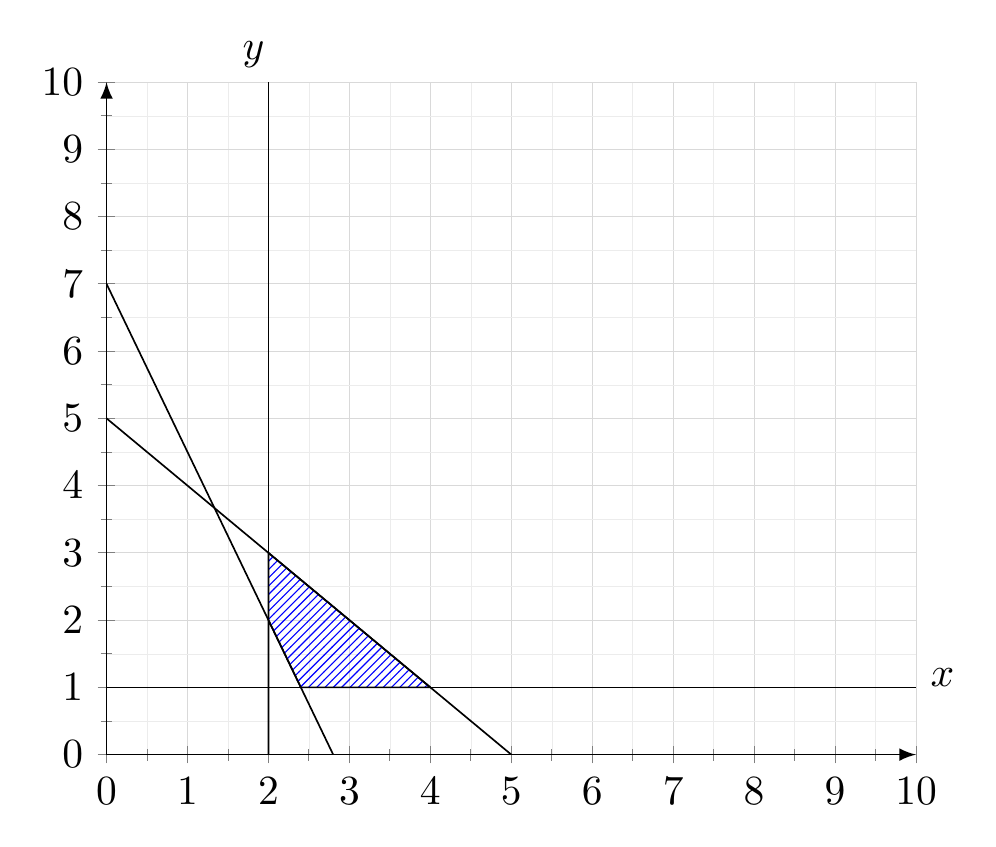
\begin{tikzpicture}[scale=1.5]
		\begin{axis}
		[
		xmin=-0,xmax=10,
		ymin=0,ymax=10,
		grid=both,
		grid style={line width=.1pt, draw=darkgray!10},
		major grid style={line width=.2pt,draw=darkgray!20},
		axis lines=left,
		minor tick num=1,
		enlargelimits={abs=0},
		axis line style={-latex},
		samples=100,
		domain = -20:20,
		ytick={0,1,...,10},
		xtick={0,1,...,10},
		xlabel={$x$},
		ylabel={$y$},
		x label style={at={(axis description cs:1,0.15)},anchor=north west},
		y label style={at={(axis description cs:0.15,1)},anchor=south west, rotate=-90}
		]
		
		\addplot [mark=dot] coordinates{(5, 0)  (0,5)} {};
		
		\addplot [mark=dot] coordinates {(2.8,0) (0, 7)} {};
		
		\addplot [mark=dot] coordinates {(2,0) (2, 10)} {};
		
		\addplot [mark=dot] coordinates {(0, 1) (10, 1)} {};
		
		\addplot [pattern=north east lines,pattern color=blue] coordinates {(2,2) (2, 3) (4, 1) (2.4,1) (2,2)} \closedcycle;	
		
		\end{axis}	
	\end{tikzpicture}
	
\end{document}